\begin{prob}

    Consider a \emph{breadth}-first search on the graph shown in the figure, starting with node $c$.

    \begin{center}
        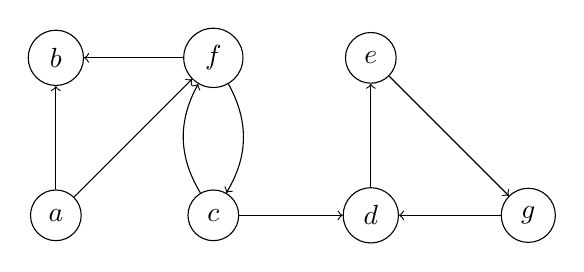
\begin{tikzpicture}
        \tikzset{
            vertex/.style={draw, circle, text width=8, align=center},
            arc/.style={->}
            }
            
            \draw node[vertex] (a) at (0,0) {$a$};
            \draw node[vertex] (b) at (0,2) {$b$};
            \draw node[vertex] (c) at (2,0) {$c$};
            \draw node[vertex] (f) at (2,2) {$f$};
            \draw node[vertex] (d) at (4,0) {$d$};
            \draw node[vertex] (e) at (4,2) {$e$};
            \draw node[vertex] (g) at (6,0) {$g$};
            \foreach \x/\y in {%
                a/b,a/f,d/e,e/g,f/b,g/d,c/d%
                }{
                    \draw (\x) edge[arc] (\y);
                }
            
            \draw (c) edge[arc, bend left] (f);
            \draw (f) edge[arc, bend left] (c);
        \end{tikzpicture}
    \end{center}
    
     \begin{subprobset}
        \begin{subprob}
            Suppose you call bfs\_shortest\_paths(graph,
            'c') on the graph above. This function returns dictionaries distance and predecessor. Write down the
            contents of these dictionaries as they are when the function exits.
            
            \begin{figure}[h!]
                \inputminted{python}{\thisdir/include/bfs_shortest_path.py}
            \end{figure}
            
            \begin{soln}
                 \\
                distance:
                \{
                \\
                'a':$\infty$,
                \\
                'b':2,
                \\
                'c':0,
                \\
                'd':1,
                \\
                'e':2,
                \\
                'f':1,
                \\
                'g':3
                \\
                \}
                \\
                predecessor:\{
                \\
                'a':None,
                \\
                'b':'f',
                \\
                'c':None,
                \\
                'd':'c',
                \\
                'e':'d',
                \\
                'f':'c',
                \\
                'g':'e'
                \\
                \}
		
            \end{soln}
        \end{subprob}
        
        \begin{subprob}
            Mark the BFS trees produced on executing BFS on this graph.
            \begin{soln}
                 \begin{center}
        	    	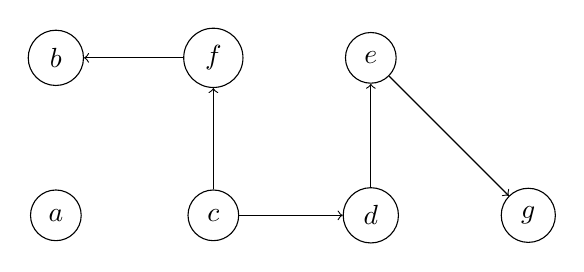
\begin{tikzpicture}
            		    \tikzset{
               			vertex/.style={draw, circle, text width=8, align=center},
        		        	arc/.style={->}
            		    }
        
               		    \draw node[vertex] (a) at (0,0) {$a$};
                		    \draw node[vertex] (b) at (0,2) {$b$};
               		    \draw node[vertex] (c) at (2,0) {$c$};
            	            \draw node[vertex] (f) at (2,2) {$f$};
                		    \draw node[vertex] (d) at (4,0) {$d$};
            		    \draw node[vertex] (e) at (4,2) {$e$};
              	    	    \draw node[vertex] (g) at (6,0) {$g$};
            		    \foreach \x/\y in {%
            			    d/e,e/g,f/b,c/d, c/f%
            		    }{
                   		 	\draw (\x) edge[arc] (\y);
           		        }

	            	\end{tikzpicture}
                \end{center}
            \end{soln}
        \end{subprob}
    \end{subprobset}
        
\end{prob}
